\chapter{Operating Lifecycle and State Coordination}
\label{chap:lifecycle}
% Traceability: ADR-002 ADR-003 ADR-004 ADR-006

The controller contains several independent boards, but an instrument must still start, arm, acquire data, stop, and recover as one system. The architecture provides a common externally visible lifecycle for this purpose.

The lifecycle does not require every board to use identical FPGA/CPLD code or identical internal states. It defines what the host and the other boards can observe. Each board remains responsible for its own readiness, local work, and fault evidence. The main board coordinates only the shared actions.

\section{Distributed Coordination}

The host, main board, and function boards have separate responsibilities:

\begin{itemize}
  \item The \textbf{host} knows the instrument configuration, sends operational settings, requests system actions, and gathers status.
  \item The \textbf{main board} drives the shared \texttt{EN}, \texttt{CLEAR}, \texttt{CLOCK}, and \texttt{SYNC} signals and observes shared health.
  \item Each \textbf{function board} checks its own readiness, controls its detector function, and enters the common safe response when required.
\end{itemize}

Before arming, the host verifies that board configuration and readiness match the intended operation. For example, a host may configure sequences and bias or clock voltages while disarmed, disconnect, and be replaced by another host. The new host may use the retained configuration after verifying that it matches the intended operation; a change of host does not itself require a reload or an interlock trip. The ICD defines the verification method.

There is no separate backplane readiness bus. The host reads readiness over the network. During arming, each function board also checks its own conditions before it allows local detector-facing permission.

This arrangement keeps coordination common without making the main board responsible for the internal operation of every function board.

\section{The Four State Families}

Every active board presents behavior consistent with four state families: \texttt{START}, \texttt{IDLE}, \texttt{RUN}, and \texttt{ERROR}. Figure~\ref{fig:state-families} shows the main transitions.

\begin{figure}[htbp]
  \centering
  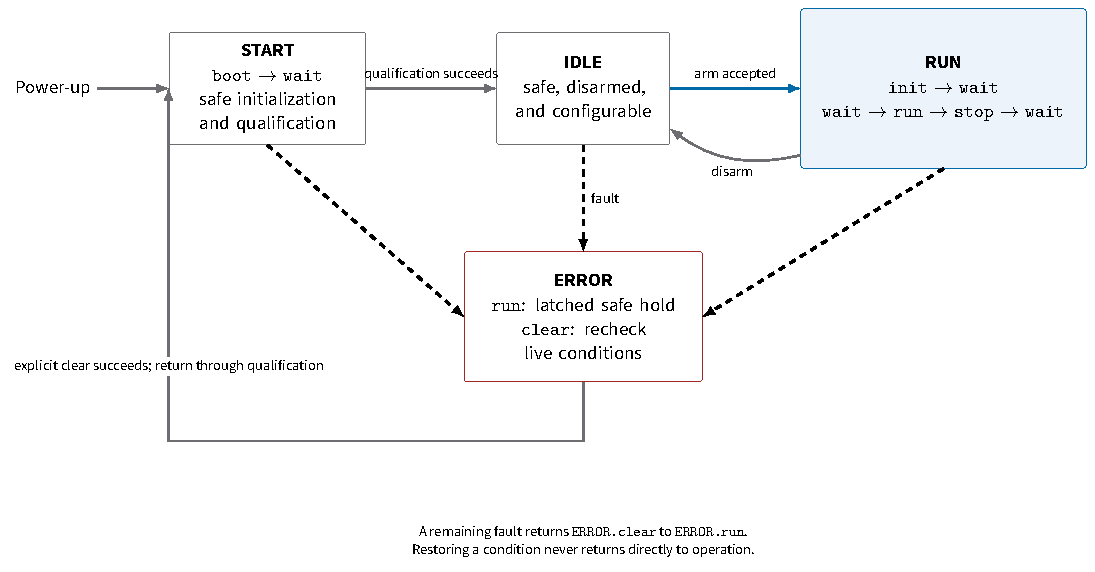
\includegraphics[width=\textwidth]{figures/generated/state_families.tikz.pdf}
  \caption{Common state families and externally visible transitions. Internal implementation may differ between boards.}
  \label{fig:state-families}
\end{figure}

\begin{table}[htbp]
\centering
\begin{tabularx}{\textwidth}{@{}>{\bfseries\raggedright\arraybackslash}p{0.20\textwidth}>{\raggedright\arraybackslash}X@{}}
\toprule
State family & Meaning \\
\midrule
\texttt{START} & The board initializes in a safe condition and then qualifies the power, timing, communication, monitoring, and shared health that apply to its role. \\
\texttt{IDLE} & The board is safe, disarmed, and available for allowed configuration. Detector protection relays remain open. \\
\texttt{RUN} & The controller is armed. The board prepares for acquisition, waits for timing events, performs its local work, and completes any controlled stop work. \\
\texttt{ERROR} & The board is held safe with fault evidence available. Recovery requires an explicit request and a new qualification pass. \\
\bottomrule
\end{tabularx}
\caption{Externally visible meaning of the common state families.}
\label{tab:state-families}
\end{table}

The state names describe system behavior rather than one mandatory state encoding. A simple board may implement fewer internal steps. A complex video or clock board may need extra local substates. Both are acceptable if their external behavior matches the common lifecycle.

\section{Safe Startup and Qualification}

At power-up, boards enter \texttt{START.boot}. Detector-facing outputs remain disabled. Each board establishes safe defaults, reads its identity, starts communication, and enables local monitoring.

The board then enters \texttt{START.wait}. In this stage it checks the live conditions needed for safe operation. Depending on the board role, these checks may include stable shared health, valid local power, required timing activity, watchdog operation, and communication readiness.

Startup qualification is bounded. A missing clock or a rail that never becomes valid cannot leave the system waiting forever and still appear usable. The applicable ICD defines the deadline and the required stable-health interval.

Boards may hold the shared \texttt{OK} bus low while their independent protection paths initialize. The system cannot reach the armable condition until required participants have released their contributions and health remains stable. A known local safety fault sends the affected board to \texttt{ERROR} instead of \texttt{IDLE}.

Successful qualification leads to \texttt{IDLE}. This is the normal safe state for configuration and inspection.

\section{Configuration in IDLE}

Operational settings are loaded while the controller is safely disarmed. Examples include detector biases, clock parameters, acquisition settings, enable masks, and sequencer data. These values are current-session information sent over Ethernet. They are separate from persistent board identity and bootstrap-network data.

Sequencer payloads are also volatile. A sequencer board remains Not Ready until the host completes the required loading transaction. If the payload is later changed, the board returns to Not Ready until the new transaction completes.

This leads to an important distinction:

\begin{table}[htbp]
\centering
\begin{tabularx}{\textwidth}{@{}>{\bfseries\raggedright\arraybackslash}p{0.22\textwidth}>{\raggedright\arraybackslash}p{0.36\textwidth}>{\raggedright\arraybackslash}X@{}}
\toprule
Condition & Meaning while disarmed & Result \\
\midrule
Not Ready & A required operational step is incomplete, but no hazardous failure is present & Arming is blocked; the board remains safe and can normally be configured \\
Fault & A safety-related hardware or electrical condition has been detected & The board asserts its trip as required and enters the latched safe error state \\
\bottomrule
\end{tabularx}
\caption{Not Ready prevents operation; Fault requires the interlock response.}
\label{tab:not-ready-fault}
\end{table}

A board that has not received a sequencer is Not Ready, not necessarily faulty. A missing required rail or a failed watchdog is a fault. Keeping these meanings separate avoids turning ordinary configuration work into a hardware trip.

Operational writes are rejected outside the safe states defined by the communication and board ICDs. Reset or power loss restores safe defaults and clears volatile sequencer readiness. A normal arm and disarm cycle does not by itself erase valid current-session settings.

\section{Distributed Arming}

The host begins arming by sending a request to the main board. Main accepts the request only from \texttt{IDLE} and only after its own requirements are satisfied. It then raises the shared \texttt{EN} signal.

Raising \texttt{EN} is not enough to force a function board to operate. Each function board independently checks its applicable conditions. These can include valid local settings, loaded sequencer data, stable power and timing, no retained fault, and a valid hardware interlock.

If the checks pass, the board enters \texttt{RUN.init} and prepares its local function. It then asserts its own local arm request and reaches \texttt{RUN.wait}. Only the combination of local permission, \texttt{EN}, and \texttt{OK} can energize the detector protection relay described in Chapter~\ref{chap:safety}.

If a board detects an unsafe arm attempt, it uses its normal local trip path. The controller returns to the shared safe response. This is stronger than allowing the system to run with one required board silently unarmed.

The main board waits through an arm-to-first-trigger guard before sending the first acquisition event. This gives every installed board enough time to recognize \texttt{EN} and complete its verified \texttt{RUN.init} work. The ICD defines the guard from the slowest supported board behavior.

\section{Acquisition Within RUN}

The \texttt{RUN} family separates arming from an individual acquisition:

\begin{itemize}
  \item \texttt{RUN.init} performs local arm-entry preparation;
  \item \texttt{RUN.wait} remains armed and waits for an acquisition event;
  \item \texttt{RUN.run} performs the timing-sensitive acquisition work; and
  \item \texttt{RUN.stop} completes the board-specific controlled stop before returning to \texttt{RUN.wait}.
\end{itemize}

A rising acquisition \texttt{SYNC} event starts the acquisition action. A falling event stops it. The exact detector clocks, sample sequence, buffering, and data framing remain local to the applicable function boards.

After \texttt{RUN.stop}, the controller may remain armed in \texttt{RUN.wait} for another acquisition. It does not need to return to \texttt{IDLE} between every exposure or readout.

Acquisition traffic may also provide the qualifying host interaction described in Chapter~\ref{chap:identity-data}.

Figure~\ref{fig:operating-sequence} shows the main interactions in a normal cycle. It represents one logical sequence, not exact protocol messages.

\begin{figure}[htbp]
  \centering
  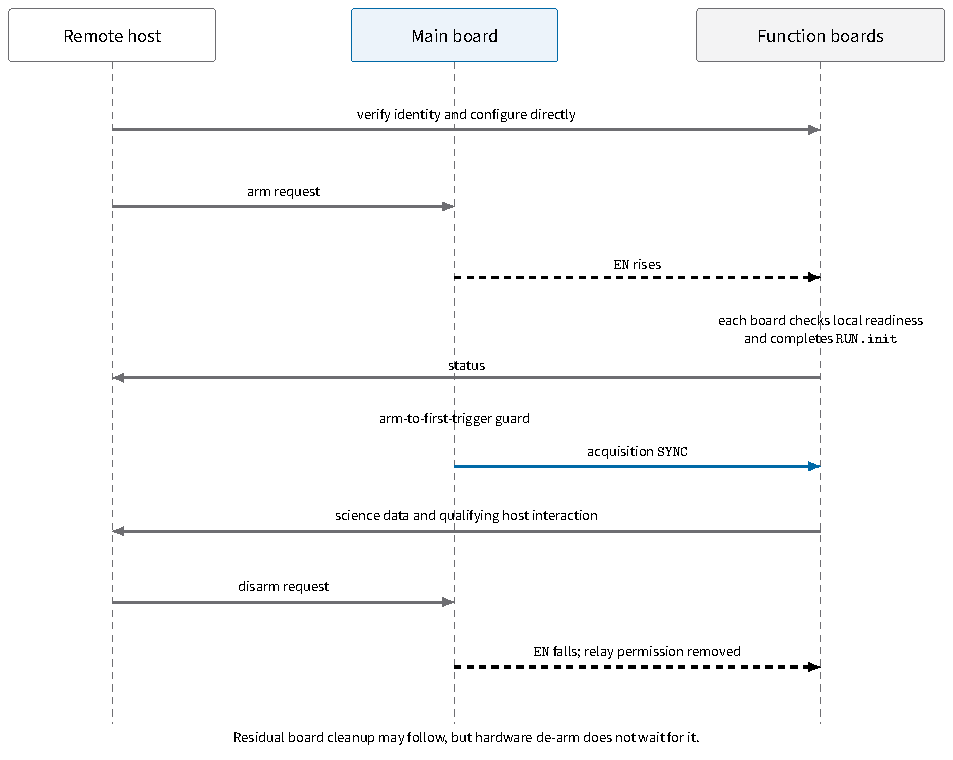
\includegraphics[width=0.92\textwidth]{figures/generated/operating_sequence.tikz.pdf}
  \caption{Normal configuration, arm, acquisition, and disarm sequence. Host communication with function boards is direct.}
  \label{fig:operating-sequence}
\end{figure}

\section{Hardware-First Disarm}

To disarm, the host asks the main board to drop system enable. This differs from stopping an acquisition while remaining armed. Main drops \texttt{EN}. The falling level removes function-board relay permission through hardware. This action does not wait for a processor response or for the board FSM to complete cleanup.

Boards then perform any remaining local cleanup and return to \texttt{IDLE}. The difference is important: the hardware becomes safe first, and orderly software or firmware cleanup follows.

\section{Fault Entry}

A detected local fault causes the affected board to assert its contribution to \texttt{OK} and retain evidence. The low shared bus removes detector-facing permission across the controller. Boards enter \texttt{ERROR.run}, where they remain safe and make diagnostics available when communication still works.

A board may enter \texttt{ERROR} because another participant tripped. It does not pull \texttt{OK} low merely because it observed the shared bus low. If it later detects its own local fault, however, it records and asserts that fault as well.

Fault entry has priority over commanded operation in \texttt{START}, \texttt{IDLE}, or any \texttt{RUN} substate. Chapter~\ref{chap:safety} describes the hardware paths that make this response independent of normal state progress.

\section{Explicit Recovery}

Recovery begins only after the controller is safe and the cause has been investigated. The host sends a clear request to the main board, and main drives the shared \texttt{CLEAR} signal.

Each locally faulted board enters \texttt{ERROR.clear} and checks its live conditions. \texttt{CLEAR} is a request, not a command to declare health. A board whose fault remains active keeps its trip asserted and returns to \texttt{ERROR.run}.

When local clearing succeeds, the system returns through \texttt{START.wait}. Required timing and shared health are qualified again before \texttt{IDLE}. There is no direct path from \texttt{ERROR} to \texttt{IDLE}, and there is never an automatic return to \texttt{RUN}.

Valid current-session operational settings do not have to be erased by ordinary fault recovery. A board may require reconfiguration when its local failure or reset invalidated those settings. Its readiness status tells the host what must be loaded again before the next arm.

\section{Armed Host Supervision}

Continued armed operation with an unavailable or unresponsive host is not assumed safe. A board need not determine whether the host froze or its communication path failed before initiating a shared trip.

Host supervision is active while \texttt{EN=1}. Every active board, including main and function boards, requires a qualifying bidirectional host interaction within a bounded interval. If the interval expires, that board records a supervision event, asserts its local trip, and places the system in the safe error state.

While disarmed (\texttt{EN=0}), loss of host contact alone does not assert \texttt{OK}. Hardware protection remains active. Data overrun alone also does not cause a trip. Chapter~\ref{chap:identity-data} explains qualifying interactions and their coexistence with science traffic.

\section{Timing Categories Belong in ICDs}

The lifecycle requires bounded timing, but this handbook does not assign numerical values. The system and board ICDs define the values from verified hardware and operational needs.

The main categories include startup deadline, stable-health qualification, clock qualification, clear pulse and recovery time, arm-to-first-trigger guard, host-supervision timeout, watchdog timing, and any required converter settling time.

Keeping the categories in the architecture ensures that important behavior is bounded. Keeping the values in ICDs allows them to change when hardware and instrument requirements become known without rewriting the system architecture.

\medskip
\noindent\textit{Chapter sources:} ADR-003 defines the common state families, arming, fault entry, disarm, and recovery. ADR-002 defines configuration and sequencer readiness. ADR-004 defines acquisition timing ownership, and ADR-006 defines data-path interaction with armed host supervision.
